%
\chapter{Omejitve GNSS v praksi}
\label{Vaje:GnssPraks} % Always give a unique label
% use \chaptermark{}
% to alter or adjust the chapter heading in the running head

Kratica GNSS zajema svetovne satelitske navigacijske sisteme: GPS, GLONASS, Beidou in Galileo. V tej nalogi boste spoznali nekaj praktičnih težav sprejema GNSS in iz njih izhajajoče možne napačne razlage navigacijskih rešitev. Glede na možnosti in okoliščine boste opazovali in dokumentirali obnašanje sprejemnika v obdobju naravnih in umetno povzročenih motenj.

\begin{figure}
	\centering
	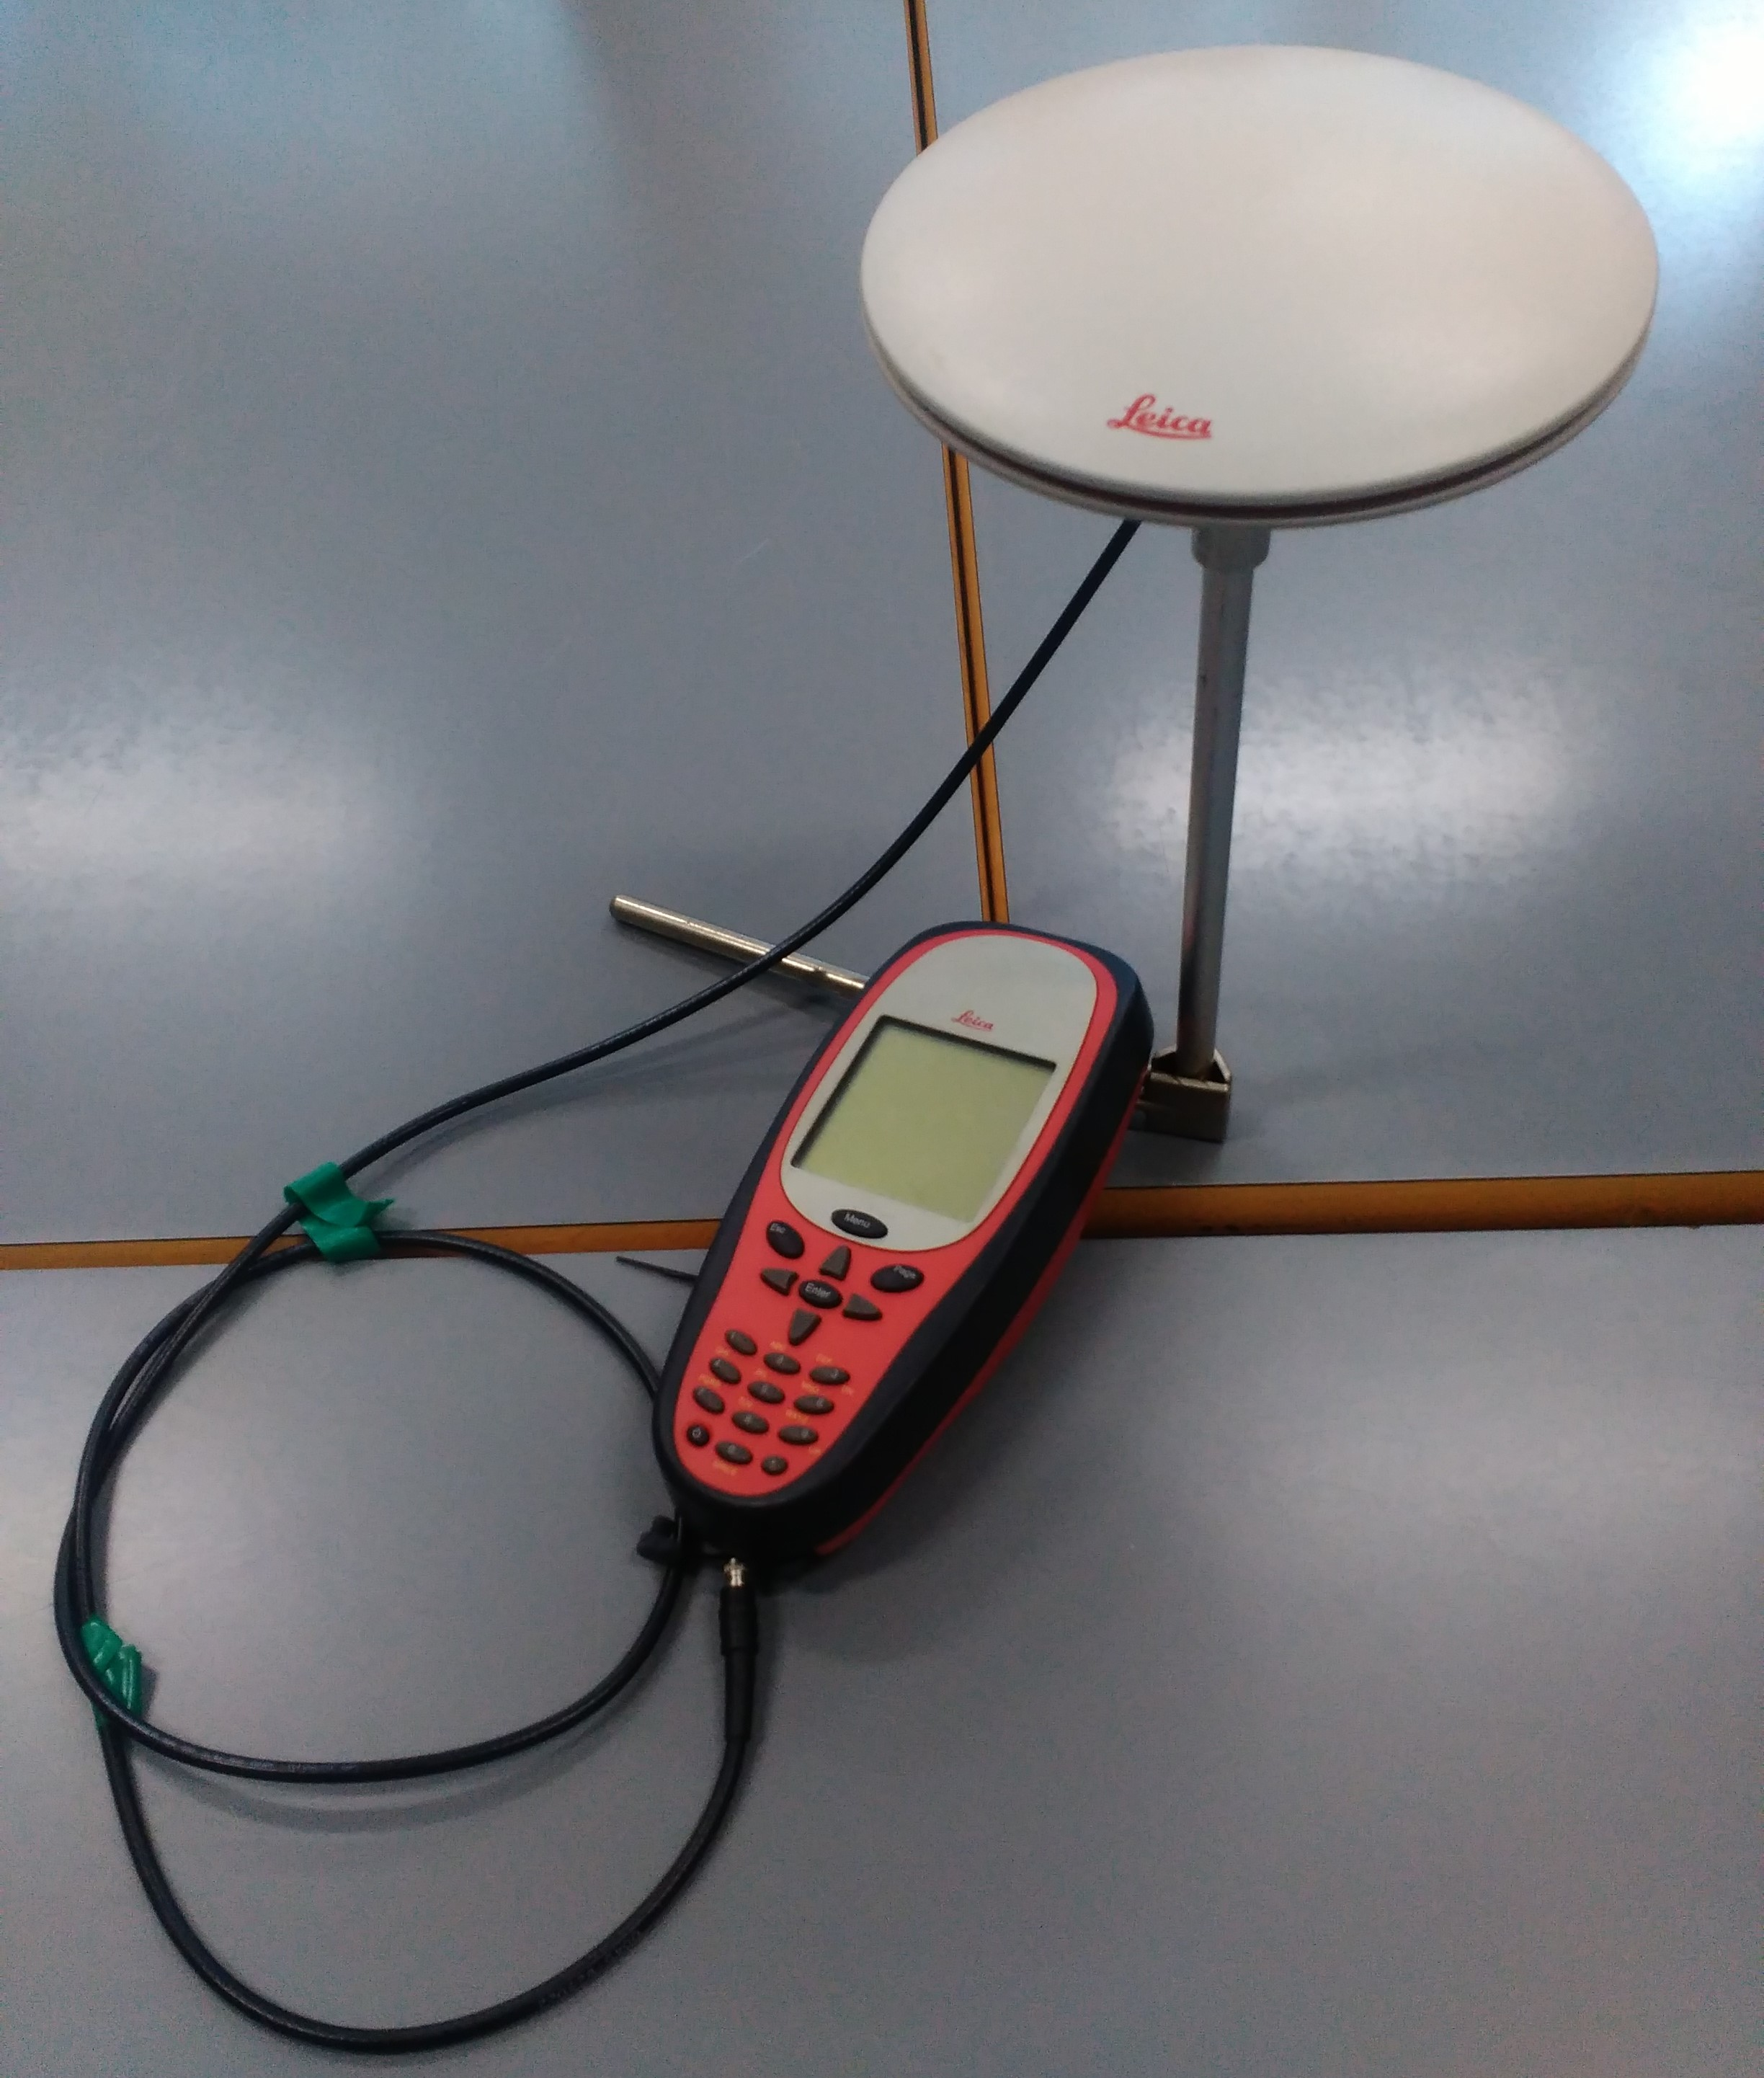
\includegraphics[height=5cm]{Vaje/OmejGnssPrak/figs/SR20-Leica.jpg}
	\caption{Eden od sprejemnikov, ki so vam na voljo. SR-20, Leica}%Gpsmap60CS, Garmin}
	\label{fig:OmejGnss_60cs}
\end{figure}

\section{Pomen naloge}
\label{sec:GnnsPomen}

Zastavite si vprašanje: Koliko lahko zaupam svojemu sprejemniku GPS? Popolnoma? V katerih pogojih lahko navigacijski rešitvi naprave bolj zaupam, kdaj manj in kdaj sploh ne?

Vsak uporabnik navigacijskega sprejemnika je že opazil, da njegov sprejemnik včasih lažje, včasih težje določi svoj položaj. Okoliščine, ki povzročajo povečanje negotovosti položaja, kako sistem sploh deluje, kakšne razsežnosti ima njegova uporaba, kaj .., boste našli v literaturi in kot \textit{razbijalci urbanih legend} praktično preverili, ali v resnici držijo ali ne.  

Koliko bi danes verjeli svoji napravi, ki uporablja satelitski način določanja položaja, če bi 8. marca 2012 prebrali v \href{http://www.bbc.com/news/technology-17119768}{\textit{članku}}:
\begin{verbatim}
"A very, very low power jammer that broadcasts on the same 
radio frequency as the GPS will drown it out.
"Most of them are used by people who don't want their vehicles 
to be tracked," he said. But the jamming technology can cause 
problems for other safety-critical systems using GPS. 
In mobile phone and power networks GPS satellite signals are 
sometimes used as a source of accurate timing information.
GPS is even used to provide accurate time information for 
some computerised transactions in financial markets. 
And other GPS navigation devices used by ships and light 
aircraft could also be affected by jammers.
\end{verbatim}

\section{Vloge v skupini}
\label{sec:Gnss_Vloge}
Skupino sestavljate vsaj štirje člani, ki si med seboj tudi pomagate, vendar vsak nosi odgovornost za svoj del.

\begin{table}
	\centering
	\caption{Oris vlog skupine Omejtve GNSS v praksi}
	\label{tab:GnssVloge} 
	\begin{tabular}{c|c|l}
		\hline\noalign{\bigskip}
		število & odgovornost                 & rezultat dela \\
		\noalign{\smallskip}\hline\noalign{\smallskip}
		2       & iskalec literature          & preizkus legend\\
		2       & priprava in izvedba poskusa & razumevanje poskusa \\
		1       & predstavitev                & izvleček izvirnega dela skupine \\ \hline
		vsi     & poročilo                    & poglobitev razumevanja vesoljskega vremena\\
		\noalign{\smallskip}\hline
	\end{tabular}
\end{table}

\subsection{Preizkus legend}
\label{subsec:GnssPrak_LitPreizkusLegend}

V desetih stavkih imate zapisanih deset govoric oz. urbanih legend, ki so zelo zakoreninjene. S študijem literature boste govorice poskusili ali potrditi ali ovreči.

\begin{enumerate}
	\item GNSS je ladijska navigacijska naprava.
	\item GNSS zagotavlja samo podatek o položaju.
	\item GPS omogoča uporabo satelitskih slik.
	\item GPS od satelita dobi informacijo kje smo.
	\item GPS je \textit{veliki brat}, ki dopušča možnost sledenja vsega in vsakogar.
	\item GNSS sateliti so geostacionarni, tako kot telekomunikacijski.
	\item Vojaški sprejemniki GPS so bolj natačni kot civilni.
	\item Uporaba GPS je dovoljena, ko plačamo uporabnino.
	\item GNSS deluje povsod.
	\item Sistem Galileo bo kmalu deloval.
\end{enumerate}

\begin{figure}
	\centering
	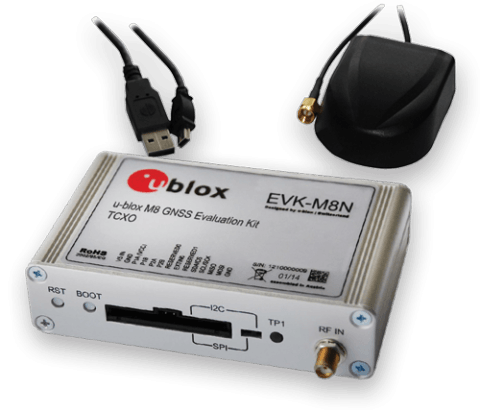
\includegraphics[height=5cm]{Vaje/OmejGnssPrak/figs/EVK-M8_withcable_trans.png}
	\caption{Eden od sprejemnikov, ki so vam na voljo. M8, u-blox}
	\label{fig:OmejGnss_ubloxM8}
\end{figure}

\textbf{Nasvet} Bodite praktični. Razmislite kaj boste v sklepih napisali o teh zakoreninjenih izrekih in kako boste z meritvami vsaj tri govorice potrdili ali ovrgli.

% NASA video 'ScienceCasts: NASA Spacecraft takes Space GPS to New Heights' iz katerega boste spoznali 'magnetic reconnection' https://www.youtube.com/watch?v=taMzKcehfGw

%tukaj je JRCjeva aplikacija za spremljanje prisotnih wi-fi omrežij, hitrosti prenosov...
% Lahko nastavita kako pogosto bosta oddajali opažanja.
% https://play.google.com/store/apps/details?id=ec.europa.eu.smartmonitor

%Andrej Štern (diapozitivi) 
%\verb|http://www.s50e.si/wp-content/uploads/2012/10/S50E-55LET-S57BAJ.pdf|

%Marko Munih: Prednosti SDR tehnologije na KV in UKV


\subsection{Sestavite pregled kritičnih okoliščin GNSS navigacije}
\label{subsec:GnssPrak_Podat}
Katere okoliščine sploh vplivajo na določanje položaja - na njegovo točnost, integriteto, neprekinljivost in dostopnost? Na katere okoliščine določanje položaja imate vpliv in na katere ne?

\subsection{Potrdite ali ovrzite vpliv kritičnih okoliščin}
\label{subsec:GnssPrak_Posk}
Načrtajte poskuse, s katerimi boste ugotovili kdaj na določanje položaja bolj vplivajo okoliščine na katere imate vpliv in kdaj bolj okoliščine na katere nimate neposrednega vpliva?
Nekatere za navigacijo pomembne okoliščine so napovedljive: 


\begin{verbatim} 
http://www.trimble.com/gnssplanningonline/#/SatLibrary
http://www.trimble.com/gnssplanningonline/#/NumSats
http://www.trimble.com/gnssplanningonline/#/Elevation
http://www.trimble.com/gnssplanningonline/#/Dops
http://www.trimble.com/gnssplanningonline/#/SatelliteVisibility
http://www.trimble.com/gnssplanningonline/#/SkyPlot
http://www.trimble.com/gnssplanningonline/#/WorldView
http://www.trimble.com/gnssplanningonline/#/IonoMap
http://www.trimble.com/gnssplanningonline/#/IonoInformation
\end{verbatim}
 

\subsection{Oprema}
\label{subsec:GnssPrak_Oprema}
V laboratorijski opremi izberite dva različna sprejemnika GNSS.


\section{Viri}
\label{sec:GnssPrak_Viri}

Pregled virov, iz katerih lahko začnete črpati snov in vaše razbijalske scenarije.

\begin{itemize}
\item {\textit{GPS locate, communicate, accelerate Essentials of Satellite Navigation Compendium}} {\tiny \begin{verbatim} https://www.u-blox.com/sites/default/files/products/documents/GPS-Compendium_Book_(GPS-X-02007).pdf \end{verbatim}} 
\item {\textit{Basics of the GPS Technique: Observation Equations}} {\tiny \begin{verbatim} http://www.nbmg.unr.edu/staff/pdfs/blewitt basics of gps.pdf\end{verbatim}}  
\item {\textit{GPS and the Quest for Pizza}} {\tiny \begin{verbatim}  http://spaceplace.nasa.gov/gps-pizza/en/\end{verbatim}}
\item {\textit{GNSS: The New GPS}} {\tiny \begin{verbatim} http://gpsworld.com/gnss-the-new-gps/ \end{verbatim}}
\item {\textit{SaPPART White paper Better use of Global Navigation Satellite Systems for safer and greener transport}} {\tiny \begin{verbatim} http://www.sappart.net/wp-content/uploads/2014/08/White-Paper_SaPPART_sept15.pdf \end{verbatim}}
\item {\textit{GNSS has bad days, too}} {\tiny \begin{verbatim} http://gpsworld.com/gnss-has-bad-days-too/ \end{verbatim}}
\item {\textit{GNSS Receiver Manufacturers Thwart Jamming, Spoofing Users on ION panel want certification requirement.}} {\tiny \begin{verbatim}  http://www.insidegnss.com/node/4684 \end{verbatim} }
\item {\textit{Tiny Device Allows You To Track Your Vehicle Using Your Smartphone}} {\tiny \begin{verbatim}   http://www.studylifestyle.com/2016/trackr/10/?cid=24&utm_term=businessinsider&sxid=9afkhwieuz44 \end{verbatim}}
\item {\textit{Using Tactical and MEMS Grade INS to Protect Against GNSS Spoofing in Automotive Applications}} {\tiny \begin{verbatim} http://gpsworld.com/automotive-absctract-ins-to-protect-against-gnss-spoofing/
\end{verbatim}}
\end{itemize}
% For built-in environments use
%
% Problems or Exercises should be sorted chapterwise
\section*{Naloge}
\addcontentsline{toc}{section}{Problems}
\begin{prob}
	\label{Nal:GnssPrak_Izvl}
	\textbf{Izvleček naj bo uvod v poročilo}\\
	(a) V skupini najdite največ pet preverljivh okoliščin, ki naj bi povečevale negotovost odčitavanja.\\
	(b) Zapišite izvleček, s katerim boste preverjali.
\end{prob}

\begin{prob}
	\label{Nal:GnssPrak_Belez}
	\textbf{Beležite podatke }\\
	(a) Izberite katere podatke o stanju in napovedih boste beležili.\\
	(b) Beležite vsaj 15 dni. \\
	(c) V poročilu kritično zapišite ujemanja med napovedmi in dejanskimi pojavi.
\end{prob}

\begin{prob}
	\label{Nal:GnssPrak_Eksp}
	\textbf{Izberite tri govorice s seznama in vsako praktično preizkusite}\\
	(a) Zamislite si tri poskuse.\\
	(b) Izvedite poskuse. \\
	(c) Zabeležite rezultate.
	(č) Posvetujte se z ostalimi člani in napišite poročilo o svojih opažanjih.
\end{prob}

\begin{prob}
	\label{Nal:GnssPrak_Predst}
	\textbf{Predstavite opravljeno delo celotne skupine}\\
	(a) Pomagajte ostalim članom pri njihovem delu. \\
	(b) Poskrbite, da je skupina v stiku s predavatelji.\\
	(b) Spremljajte napredek in sestavite osnutek poročila. \\
	(č) Po oddanem poročilu pripravite 5 minutno predstavitev na tabli.
\end{prob}
%
